\section{Smart Grid -ready}


\section{Modbus}

  Modbus on automaatiossa käytetty palvelin--asiakas-mallin viestintäprotokolla. Sen on alunperin kehittänyt vuonna 1979 yritys nimeltään Modicon käytettäväksi valmistamiens ohjelmoitavien logiikoiden eli \Gls{plc}:den väliseen viestintään. Nykyin Modicon on osa Ranskalaista Schneider Electriciä. Koska standardi on julkaistu avoimesti kaikkien käytettäväksi ja se on verrattain yksinkertainen, on se saavuttanut johtavan aseman teollisuudessa. Yleisimmille ohjelmointikielille on saatavilla modbus-standardin toteuttavat kirjastot, joiden avulla voidaan ohjelmallisesti  ohjata laitteita. Laajan levinneisyyden ansiosta modbus soveltuu monien eri valmistajien laitteiden järjestelmien kanssa käytettäväksi. Teollisuuden lisäksi protokollaa käytetään myös talo- ja kiinteistöautomaatiossa.\parencite{sousaPortugal, modbusAppSpec, modbusOrg}

  Vuonna 2004 Schneider Electric siirsi modbus-standardin hallinnan voittoa tavoittelemattomalle Modbus-järjestölle\footnote{Modbus Organization, Inc}. Järjestön muodostavat automaatiolaitteita valmistavat yritykset ja yksittäiset henkilöt ja sen tehtäviin kuuluu ylläpitää ja kehittää modbus-standardia ja siihen liittyviä documentteja sekä toimia etujärjestönä edistäen modbusin käyttöä. Modbusiin liittyvien documenttien ja julkaisujen avulla edistetään eri valmistajien järjestelmien välistä kommunikaatiota ja helpotetaan niiden integraatioita toisiinsa.  \parencite{modbusOrg}

  \subsection{tietomalli ja viestintä}

  Modbus-protokollan toiminta perustuu palvelinlaitteella sijaitsevien muistialueiden lukemiseen ja kirjoittamiseen kuvassa \ref{fig:c_s} kuvatun asiakas--palvelin-mallin mukaan.  Lukemalla tietoja asiakaslaite kykenee seuraamaan palvelinlaitteen tilaa ja kirjoittamalla ohjaamaan sen toimintaa. Tietojen lukeminen ja kirjoittaminen tapahtuu protokollan määrittämien kysely, vastaus- ja virheviestien perusteella.

  \begin{figure}
    \centering
    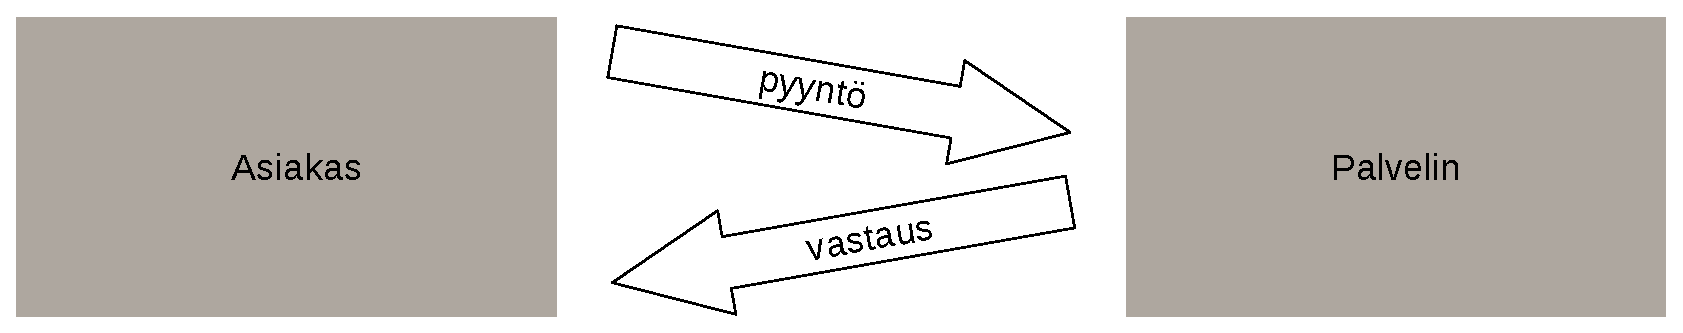
\includegraphics[width=1\textwidth]{figures/client_server}
    \caption{asiakas--palvelin-mallin}
    \label{fig:c_s}
  \end{figure}

  \subsection{funktiokoodit}
   koodeja

  \subsection{protokollan rakenne}

    Modbus-protokollasta on totetutettu muutamia eri versioita:
    \begin{itemize}
      \item sarjaväyläversio, joka muodostuu kahdesta muunnelmasta:
      \begin{itemize}
        \item Modbus RTU ja
        \item Modbus ASCII,
      \end{itemize}
      \item Modbus TCP/IP ja
      \item Modbus Plus.
      \parencite{modbusAppSpec}
    \end{itemize}
    Edellisistä Modbus Plus on Schneider Electricin hallinnoima, eikä se ole avoimesti saatavilla. Modbus Plus on oma Modbusista eroava standardinsa, jota ei tässä käsitellä enempää.\parencite{seCom}

    Taulukossa \ref{rakenne} on Modbus-protokollaperhettä verrattu \gls{OSI}-malliin. Modbus-protokollan ylempi kerros, eli viestintäkerros sijoittuu \gls{OSI}-mallissa kerroseen 7, eli sovelluskerrokseen. Sarjaväyläversiossa alempi kerros taas sijoittuu \gls{OSI}-mallissa kerrokseen 2 ja Modbus TCP/IP:n tapauksessa kerrokseen 5\footnote{\gls{OSI}-mallin teoreettisesta luonteesta johtuen tästä voinee esittää eroavia mielipiteitä.}.

    \begin{table}
      \centering
      \begin{tabular}{|c|c|ccc|}
        \hline
        \multicolumn{2}{|c|}{\gls{OSI}-mali} & \multicolumn{3}{c|}{Modbus protokollaperhe}                                         \\ \hline
        7       & sovelluskerros       & \multicolumn{3}{c|}{\gls{MBAP} (Modbus-viestintäprotokolla)}                                \\ \hline
        6       & esityskerros         &                                 &                                   &                 \\ \cline{1-2} \cline{5-5}
        5       & istuntokerros        &                                 & \multicolumn{1}{c|}{}             & Modbus-\gls{TCP}\\ \cline{1-2} \cline{5-5}
        4       & kuljetuskerros       &                                 & \multicolumn{1}{c|}{}             & \gls{TCP}       \\ \cline{1-2} \cline{5-5}
        3       & verkkokerros         &                                 & \multicolumn{1}{c|}{}             & IP              \\ \hline
        2       & siirtokerros         & \multicolumn{1}{c|}{Modbus-\gls{RTU}} & \multicolumn{1}{c|}{Modbus-\gls{ASCII}} & Ethernet, \dots \\ \hline
        1       & fyysinen kerros      & \multicolumn{2}{c|}{\gls{RS}-232 / \gls{RS}-485}                                & Ethernet, \dots \\ \hline
      \end{tabular}
      \caption[Modbus-protokollan rakenne ja \gls{OSI}-malli]{Modbus-protokollan rakenne ja sen sovitus \gls{OSI}-malliin.\parencite{osi, modbusSerialSpec, modbusTCPIPSpec}}
      \label{rakenne}
    \end{table}

    Protokollan ylempi kerros eli \gls{MBAP} on kaikille Modbus-versioille yhteinen ja se mahdollistaa viestinnän laitteiden kesken erilaisten verkkojen ylitse. Protokollan määrittelee, että \gls{MBAP} voi muodostaa kolmen tyyppisiä \gls{APDU}:ja, jotka välittävät viestejä.
